\documentclass[reqno, 12pt]{article}
\usepackage{amsmath}
\usepackage{amsfonts}
\usepackage{amssymb}
\usepackage{enumerate}
\usepackage{graphicx}
\usepackage{wrapfig}
\usepackage[mathscr]{euscript}
\usepackage{stmaryrd}
\usepackage[normalem]{ulem}
\usepackage{fullpage}
\newcommand{\R}{\mathbb{R}}
\newcommand{\Z}{\mathbb{Z}}
\newcommand{\Q}{\mathbb{Q}}
\newcommand{\N}{\mathbb{N}}
\newcommand{\Lagr}{\mathcal{L}}
\newcommand{\END}{\hspace*{\fill} $\clubsuit$}
\newcommand{\st}{\sout{$\supset$}}
\newcommand{\vx}{ \mathbf{x} }
\newcommand{\vy}{ \mathbf{y} }
\newcommand{\degree}{^\circ}
\graphicspath{graphics}

\begin{document}
I began my study with the introduction. I want to make sure I know the motiviation for the results. It seems we are interested in a few things for a function $f \,: \, \Omega \subset \R^n \rightarrow \R^n$ defined by $f(x) = y$. They are
\begin{enumerate}
\item existence of a solution for a given $x \in \Omega$,
\item uniqueness of solution,
\item distribution of all solutions in $\Omega$,
\item and knowing what happens if we change $f$ and $y$ in some way.
\end{enumerate}
We begin to discuss the winding number. The intuition I am holding on to from Deimling is the winding number "tells us how many times $\Gamma$ winds around $a$...". Here, $\Gamma$ is some closed curve that is continuously differentiable around a point $a \in \mathbb{C}\backslash\Gamma$. I looked online for more intuition of the winding number.
\begin{figure}[h]
	\centering
	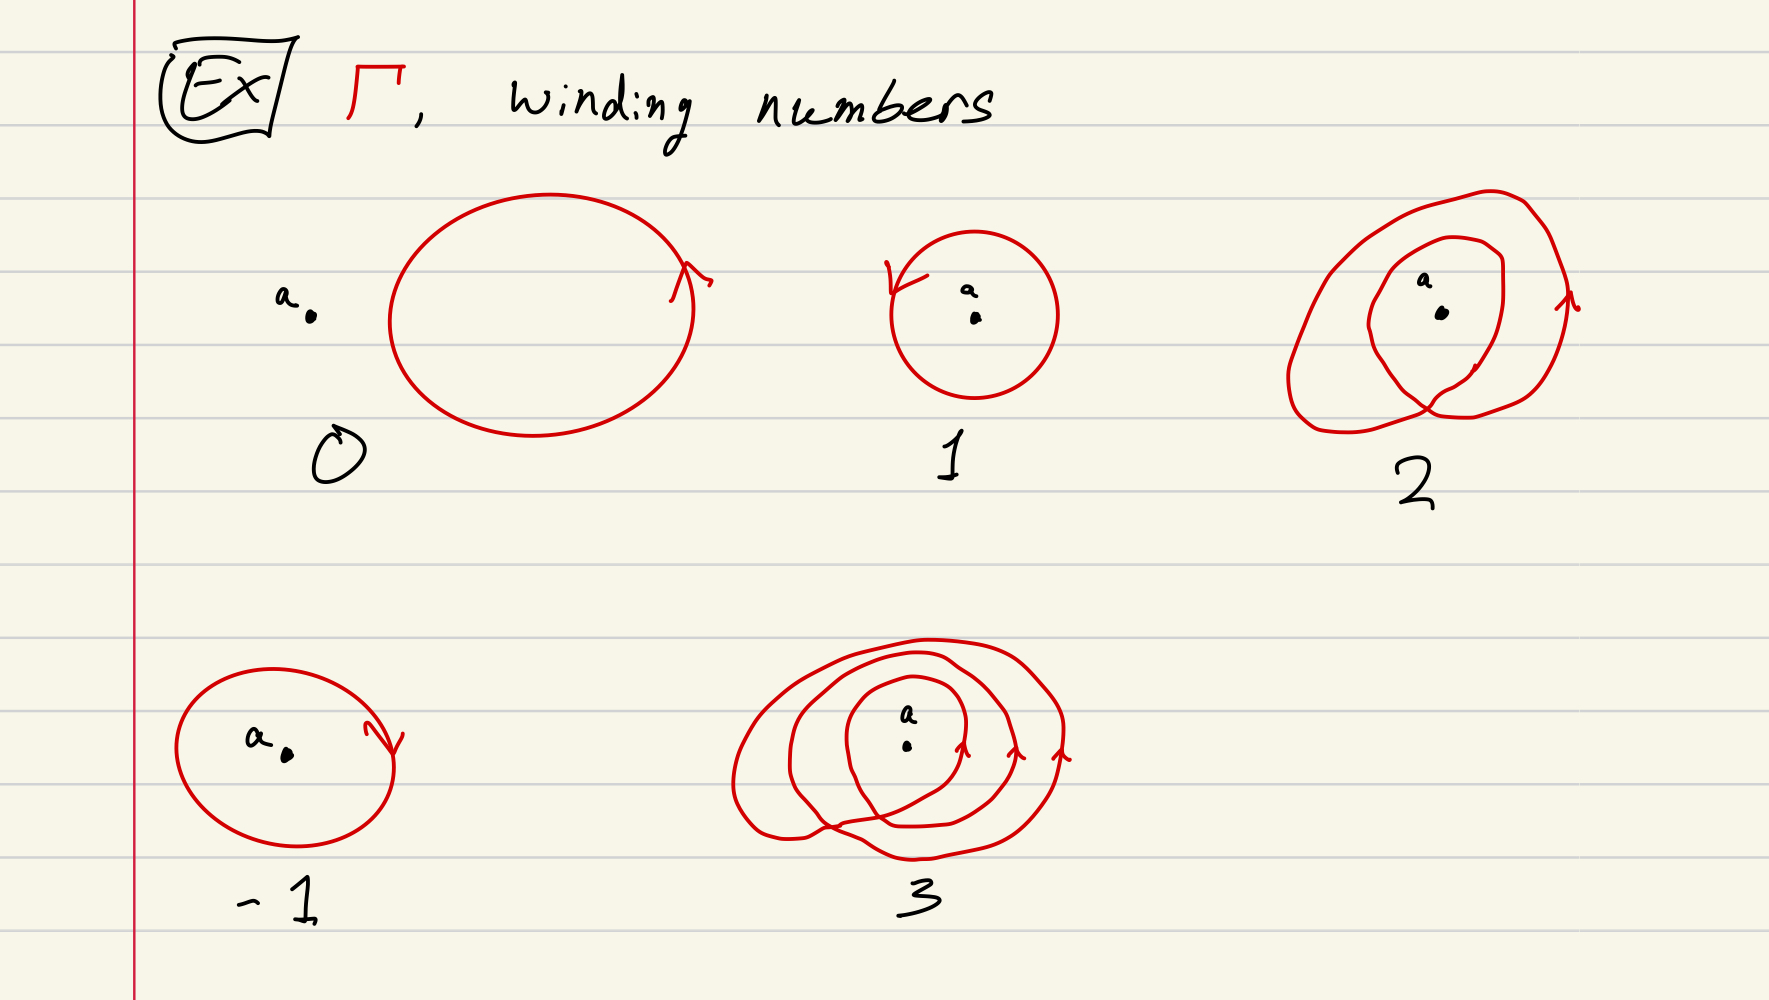
\includegraphics[width = .8 \textwidth]{winding-number-1.jpeg}
\end{figure}
Notice that $\Gamma$ is oriented with the convention being positive for counter-clockwise orientation. Since I had just finished an algebraic topology course this fall, I thought about how easy it would be to apply the winding number on a simplex. This connection to topology is important. It turns out a powerful property of the "degree" function is being homotopy invariant. More on this later.

By the end of the introduction, I had written down a few concepts I needed to review. They were: the definition of an analytic function, the Bolzano Intermediate Value Theorem (IVT), Implicit Function Theorem, and Sard's Lemma. I was least aware of the Bolzano IVT as it is a special case of the general IVT, stating the existence of a root (of a function), but not its "location", roughly speaking. 

I also realized how dense this book can be. It is taking me awhile reading through the first section and perhaps too deeply. I think I will switch strategies and read results for intuition, fill in gaps of my knowledge with the supplemental texts (as planned), and use the internet for better pictures. After some general intuition and questions are generated, then I can go back and think more carefully. 
\\\\This concludes my first post. \END
\end{document}
